\documentclass[10pt,onecolumn,letterpaper]{article}

\usepackage{cvpr}
\usepackage{times}
\usepackage{epsfig}
\usepackage{graphicx}
\usepackage{amsmath}
\usepackage{amssymb}
\usepackage{subfigure}
\usepackage{upgreek}
\usepackage{multirow}
\usepackage{color}
\usepackage{float}

% Include other packages here, before hyperref.

% If you comment hyperref and then uncomment it, you should delete
% egpaper.aux before re-running latex.  (Or just hit 'q' on the first latex
% run, let it finish, and you should be clear).
\usepackage[pagebackref=true,breaklinks=true,letterpaper=true,colorlinks,bookmarks=false]{hyperref}

% \cvprfinalcopy % *** Uncomment this line for the final submission

\def\cvprPaperID{1047} % *** Enter the CVPR Paper ID here
\def\httilde{\mbox{\tt\raisebox{-.5ex}{\symbol{126}}}}

% Pages are numbered in submission mode, and unnumbered in camera-ready
\ifcvprfinal\pagestyle{empty}\fi


\begin{document}

%%%%%%%%% TITLE
\title{Supplementary Material to ``External Prior Guided Internal Prior Learning for Real Noisy Image Denoising"}

\author{First Author\\
Institution1\\
Institution1 address\\
{\tt\small firstauthor@i1.org}
% For a paper whose authors are all at the same institution,
% omit the following lines up until the closing ``}''.
% Additional authors and addresses can be added with ``\and'',
% just like the second author.
% To save space, use either the email address or home page, not both
\and
Second Author\\
Institution2\\
First line of institution2 address\\
{\tt\small secondauthor@i2.org}
}

\maketitle


%%%%%%%%% BODY TEXT
In this supplementary material, we provide:\vspace{-0.1in}
\begin{enumerate}
\item The closed-form solution of the proposed weighted sparse coding model in the main paper.
\vspace{-0.1in}
\item More denoising results on the real noisy images (with no ``ground truth") provided in the dataset \cite{ncwebsite}.
\vspace{-0.1in}
\item More denoising results on the 15 cropped real noisy images (with ``ground truth") used in the dataset \cite{crosschannel2016}.
\vspace{-0.1in}
\item More denoising results on the 60 cropped real noisy images (with ``ground truth") from \cite{crosschannel2016}.
\end{enumerate}
\section{Closed-Form Solution of the Weighted Sparse Coding Problem (4)}
The weighted sparse coding problem in the main paper is:
\begin{equation}\label{equ1}
\setlength{\abovedisplayskip}{1pt}
\setlength{\belowdisplayskip}{1pt}
\min_{\boldsymbol{\alpha}}\|\mathbf{y}-\mathbf{D}\boldsymbol{\alpha}\|_{2}^{2}+\|\mathbf{w}^{T}\boldsymbol{\alpha}\|_{1}.
\end{equation}
Since $\mathbf{D}$ is an orthonormal matrix, problem (\ref{equ1}) is equivalent to 
\begin{equation}\label{equ2}
\setlength{\abovedisplayskip}{1pt}
\setlength{\belowdisplayskip}{1pt}
\min_{\boldsymbol{\alpha}}\|\mathbf{D}^{T}\mathbf{y}-\boldsymbol{\alpha}\|_{2}^{2}+\|\mathbf{w}^{T}\boldsymbol{\alpha}\|_{1}.
\end{equation}
For simplicity, we denote $\mathbf{z} = \mathbf{D^{T}y}$. Since $\mathbf{w}_{i}=c*2\sqrt{2}\sigma^{2}/(\mathbf{\Lambda}_{i}+\varepsilon)$ is positive (please refer to Eq. (18) in the main paper), problem (\ref{equ2}) can be written as
\begin{equation}\label{equ3}
\setlength{\abovedisplayskip}{0.01pt}
\setlength{\belowdisplayskip}{0.01pt}
\min_{\boldsymbol{\alpha}}\sum_{i=1}^{p^{2}}((\mathbf{z}_{i}-\boldsymbol{\alpha}_{i})^{2}+\mathbf{w}_{i}|\boldsymbol{\alpha}_{i}|).
\end{equation}
The problem (\ref{equ3}) is separable w.r.t. $\boldsymbol{\alpha}_{i}$ and can be simplified to $p^{2}$ scalar minimization problems
\begin{equation}\label{equ4}
\setlength{\abovedisplayskip}{2pt}
\setlength{\belowdisplayskip}{1pt}
\min_{\boldsymbol{\alpha}_{i}}(\mathbf{z}_{i}-\boldsymbol{\alpha}_{i})^{2}+\mathbf{w}_{i}|\boldsymbol{\alpha}_{i}|,
\end{equation}
where $i=1,...,p^{2}$. Taking derivative of $\boldsymbol{\alpha}_{i}$ in problem (\ref{equ4}) and setting the derivative to be zero. There are two cases for the solution.

(a) If $\boldsymbol{\alpha}_{i}\ge 0$, we have
\begin{equation}\label{equ5}
\setlength{\abovedisplayskip}{0.1pt}
\setlength{\belowdisplayskip}{0.11pt}
2(\boldsymbol{\alpha}_{i}-\mathbf{z}_{i})+\mathbf{w}_{i}=0.
\end{equation}
\qquad\ \  The solution is
\begin{equation}\label{equ6}
\setlength{\abovedisplayskip}{0.1pt}
\setlength{\belowdisplayskip}{0.1pt}
\hat{\boldsymbol{\alpha}}_{i}=\mathbf{z}_{i}-\frac{\mathbf{w}_{i}}{2} \ge 0.
\end{equation}
\qquad\ \  So $\mathbf{z}_{i}\ge\frac{\mathbf{w}_{i}}{2}> 0$, and the solution $\hat{\boldsymbol{\alpha}}_{i}$ can be written as
\begin{equation}\label{equ7}
\setlength{\abovedisplayskip}{0.1pt}
\setlength{\belowdisplayskip}{0.1pt}
\hat{\boldsymbol{\alpha}}_{i}=\text{sgn}(\mathbf{z}_{i})*(|\mathbf{z}_{i}|-\frac{\mathbf{w}_{i}}{2}),
\end{equation}
\qquad\ \  where $\text{sgn}(\bullet)$ is the sign function. 

(b) If $\boldsymbol{\alpha}_{i}< 0$, we have
\begin{equation}\label{equ8}
\setlength{\abovedisplayskip}{0.1pt}
\setlength{\belowdisplayskip}{0.1pt}
2(\boldsymbol{\alpha}_{i}-\mathbf{z}_{i})-\mathbf{w}_{i}=0.
\end{equation}
\qquad\ \  The solution is
\begin{equation}\label{equ9}
\setlength{\abovedisplayskip}{0.1pt}
\setlength{\belowdisplayskip}{0.1pt}
\hat{\boldsymbol{\alpha}}_{i}=\mathbf{z}_{i}+\frac{\mathbf{w}_{i}}{2} < 0.
\end{equation}
\qquad\ \  So $\mathbf{z}_{i}<-\frac{\mathbf{w}_{i}}{2}< 0$, and the solution $\hat{\boldsymbol{\alpha}}_{i}$ can be written as
\begin{equation}\label{equ10}
\setlength{\abovedisplayskip}{1pt}
\setlength{\belowdisplayskip}{1pt}
\hat{\boldsymbol{\alpha}}_{i}=\text{sgn}(\mathbf{z}_{i})*(-\mathbf{z}_{i}-\frac{\mathbf{w}_{i}}{2})=\text{sgn}(\mathbf{z}_{i})*(|\mathbf{z}_{i}|-\frac{\mathbf{w}_{i}}{2}).
\end{equation} 

In summary, we have the final solution of the weighted sparse coding problem (\ref{equ1}) as
\begin{equation}\label{equ11}
\setlength{\abovedisplayskip}{3pt}
\setlength{\belowdisplayskip}{3pt}
\hat{\boldsymbol{\alpha}}= \text{sgn}(\mathbf{D^{T}y})\odot \text{max}(|\mathbf{D^{T}y}|-\mathbf{w}/2,0),
\end{equation}
where $\odot$ means element-wise multiplication and $|\mathbf{D^{T}y}|$ is the absolute value of each entry of the vector $\mathbf{D^{T}y}$.



%------------------------------------------------------------------------------------
%------------------------------------------------------------------------------------

\section{More Results on Real Noisy Images in \cite{ncwebsite}}
In this section, we give more visual comparisons of the competing methods on the real noisy images provided in \cite{ncwebsite}. The real noisy images in this dataset \cite{ncwebsite} have no ``ground truth" images and hence we only compare the visual quality of the denoised images by different methods. As can be seen from Figures \ref{fig1}-\ref{fig4}, our proposed method perfomrs better than the state-of-the-art denoising methods. This validates the effectiveness of our proposed external prior guided internal prior learning framework for real noisy image denoising.

%------------------------------------------------------------------------------------
\begin{figure}[H]\vspace{2mm}
\centering
\subfigure{
\begin{minipage}[t]{0.244\textwidth}
\centering
\raisebox{-0.15cm}{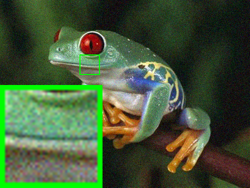
\includegraphics[width=1\textwidth]{imagessupp/resize_frog_noisy.png}}
{\footnotesize (a) Noisy \cite{ncwebsite}   }
\end{minipage}
\begin{minipage}[t]{0.244\textwidth}
\centering
\raisebox{-0.15cm}{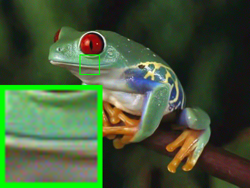
\includegraphics[width=1\textwidth]{imagessupp/resize_frog_cbm3d.png}}
{\footnotesize (b) CBM3D \cite{bm3d,cbm3d}  }
\end{minipage}
\begin{minipage}[t]{0.244\textwidth}
\centering
\raisebox{-0.15cm}{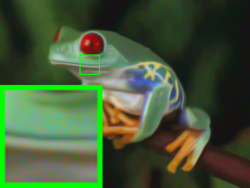
\includegraphics[width=1\textwidth]{imagessupp/resize_frog_wnnm.png}}
{\footnotesize (c) WNNM \cite{wnnm}   }
\end{minipage}
\begin{minipage}[t]{0.244\textwidth}
\centering
\raisebox{-0.15cm}{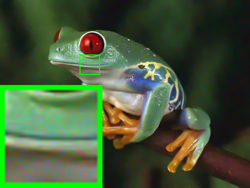
\includegraphics[width=1\textwidth]{imagessupp/resize_frog_mlp.png}}
{\footnotesize (d) MLP \cite{mlp}  }
\end{minipage}
}\vspace{-2mm}
\subfigure{
\begin{minipage}[t]{0.244\textwidth}
\centering
\raisebox{-0.15cm}{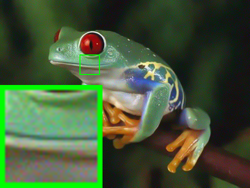
\includegraphics[width=1\textwidth]{imagessupp/resize_frog_tnrd.png}}
{\footnotesize (e) TNRD \cite{chen2015learning}}
\end{minipage}
\begin{minipage}[t]{0.244\textwidth}
\centering
\raisebox{-0.15cm}{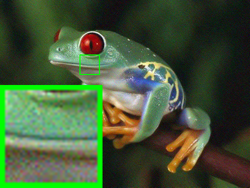
\includegraphics[width=1\textwidth]{imagessupp/resize_frog_ni.png}}
{\footnotesize (f) NI \cite{neatimage}  }
\end{minipage}
\begin{minipage}[t]{0.244\textwidth}
\centering
\raisebox{-0.15cm}{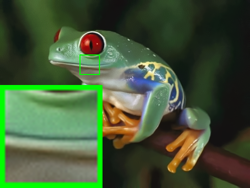
\includegraphics[width=1\textwidth]{imagessupp/resize_frog_nc.png}}
{\footnotesize (g) NC \cite{ncwebsite,noiseclinic}   }
\end{minipage}
\begin{minipage}[t]{0.244\textwidth}
\centering
\raisebox{-0.15cm}{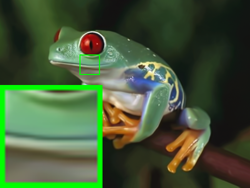
\includegraphics[width=1\textwidth]{imagessupp/resize_frog_ours.png}}
{\footnotesize (h) Ours  }
\end{minipage}
}
\caption{Denoised images of the real noisy image ``Frog" \cite{ncwebsite} by different methods. The images are better to be zoomed in on screen.}
\label{fig1}
\end{figure}

%------------------------------------------------------------------------------------
\begin{figure}[H]
\centering
\subfigure{
\begin{minipage}[t]{0.244\textwidth}
\centering
\raisebox{-0.15cm}{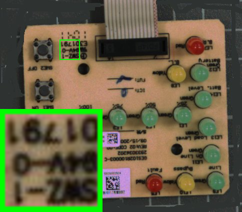
\includegraphics[width=1\textwidth]{imagessupp/resize_br_Noisy_circuit.png}}
{\footnotesize (a) Noisy \cite{ncwebsite}   }
\end{minipage}
\begin{minipage}[t]{0.244\textwidth}
\centering
\raisebox{-0.15cm}{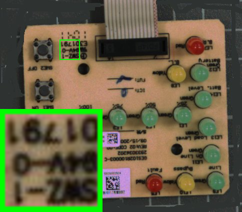
\includegraphics[width=1\textwidth]{imagessupp/resize_br_BM3D_circuit.png}}
{\footnotesize (b) CBM3D \cite{bm3d,cbm3d}  }
\end{minipage}
\begin{minipage}[t]{0.244\textwidth}
\centering
\raisebox{-0.15cm}{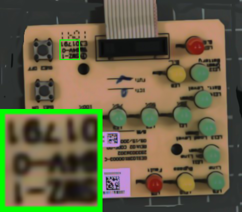
\includegraphics[width=1\textwidth]{imagessupp/resize_br_WNNM_circuit.png}}
{\footnotesize (c) WNNM \cite{wnnm}   }
\end{minipage}
\begin{minipage}[t]{0.244\textwidth}
\centering
\raisebox{-0.15cm}{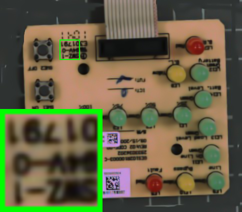
\includegraphics[width=1\textwidth]{imagessupp/resize_br_MLP_circuit.png}}
{\footnotesize (d) MLP \cite{mlp}  }
\end{minipage}
}\vspace{-2mm}
\subfigure{
\begin{minipage}[t]{0.244\textwidth}
\centering
\raisebox{-0.15cm}{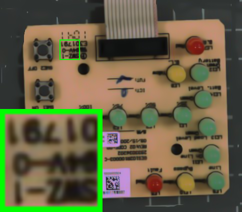
\includegraphics[width=1\textwidth]{imagessupp/resize_br_TRD_circuit.png}}
{\footnotesize (e) TNRD \cite{chen2015learning}}
\end{minipage}
\begin{minipage}[t]{0.244\textwidth}
\centering
\raisebox{-0.15cm}{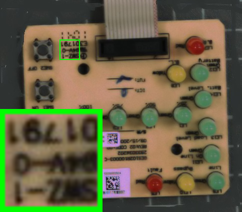
\includegraphics[width=1\textwidth]{imagessupp/resize_br_NI_circuit.png}}
{\footnotesize (f) NI \cite{neatimage}  }
\end{minipage}
\begin{minipage}[t]{0.244\textwidth}
\centering
\raisebox{-0.15cm}{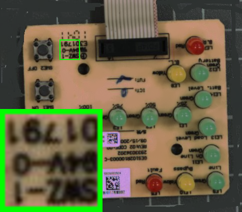
\includegraphics[width=1\textwidth]{imagessupp/resize_br_NC_circuit.png}}
{\footnotesize (g) NC \cite{ncwebsite,noiseclinic}   }
\end{minipage}
\begin{minipage}[t]{0.244\textwidth}
\centering
\raisebox{-0.15cm}{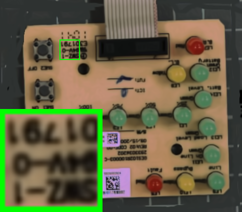
\includegraphics[width=1\textwidth]{imagessupp/resize_br_Guided_circuit.png}}
{\footnotesize (h) Ours  }
\end{minipage}
}
\caption{Denoised images of the real noisy image ``Circuit" \cite{ncwebsite} by different methods. The images are better to be zoomed in on screen.}
\label{fig2}
\end{figure}

%------------------------------------------------------------------------------------
\begin{figure}[H]\vspace{3mm}
\centering
\subfigure{
\begin{minipage}[t]{0.244\textwidth}
\centering
\raisebox{-0.15cm}{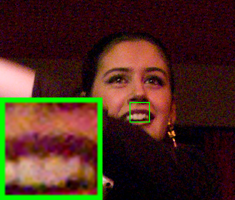
\includegraphics[width=1\textwidth]{imagessupp/resize_br_Noisy_woman.png}}
{\footnotesize (a) Noisy \cite{ncwebsite}   }
\end{minipage}
\begin{minipage}[t]{0.244\textwidth}
\centering
\raisebox{-0.15cm}{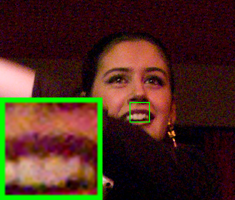
\includegraphics[width=1\textwidth]{imagessupp/resize_br_BM3D_woman.png}}
{\footnotesize (b) CBM3D \cite{bm3d,cbm3d}  }
\end{minipage}
\begin{minipage}[t]{0.244\textwidth}
\centering
\raisebox{-0.15cm}{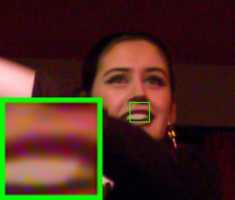
\includegraphics[width=1\textwidth]{imagessupp/resize_br_WNNM_woman.png}}
{\footnotesize (c) WNNM \cite{wnnm}   }
\end{minipage} 
\begin{minipage}[t]{0.244\textwidth}
\centering
\raisebox{-0.15cm}{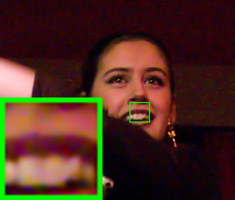
\includegraphics[width=1\textwidth]{imagessupp/resize_br_MLP_woman.png}}
{\footnotesize (d) MLP \cite{mlp}  }
\end{minipage}
}\vspace{-2mm}
\subfigure{
\begin{minipage}[t]{0.244\textwidth}
\centering
\raisebox{-0.15cm}{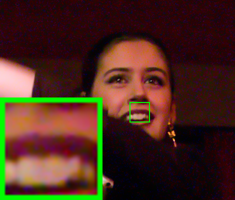
\includegraphics[width=1\textwidth]{imagessupp/resize_br_TRD_woman.png}}
{\footnotesize (e) TNRD \cite{chen2015learning}}
\end{minipage}
\begin{minipage}[t]{0.244\textwidth}
\centering
\raisebox{-0.15cm}{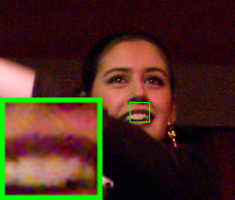
\includegraphics[width=1\textwidth]{imagessupp/resize_br_NI_woman.png}}
{\footnotesize (f) NI \cite{neatimage}  }
\end{minipage}
\begin{minipage}[t]{0.244\textwidth}
\centering
\raisebox{-0.15cm}{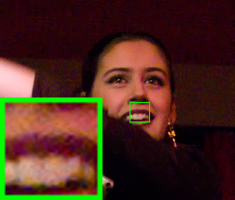
\includegraphics[width=1\textwidth]{imagessupp/resize_br_NC_woman.png}}
{\footnotesize (g) NC \cite{ncwebsite,noiseclinic}   }
\end{minipage}
\begin{minipage}[t]{0.244\textwidth}
\centering
\raisebox{-0.15cm}{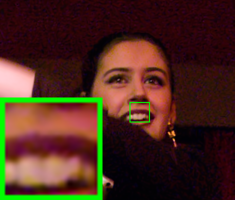
\includegraphics[width=1\textwidth]{imagessupp/resize_br_Guided_woman.png}}
{\footnotesize (h) Ours  }
\end{minipage}
}
\caption{Denoised images of the real noisy image ``Woman" \cite{ncwebsite} by different methods. The images are better to be zoomed in on screen.}
\label{fig3}
\end{figure}

%------------------------------------------------------------------------------------
\begin{figure}[H]\vspace{3mm}
\centering
\subfigure{
\begin{minipage}[t]{0.244\textwidth}
\centering
\raisebox{-0.15cm}{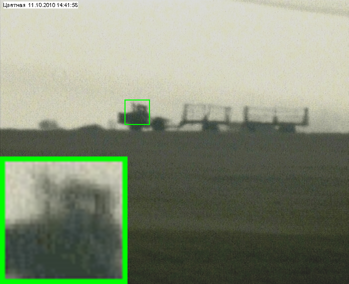
\includegraphics[width=1\textwidth]{imagessupp/resize_br_Noisy_vehicle.png}}
{\footnotesize (a) Noisy \cite{ncwebsite}   }
\end{minipage}
\begin{minipage}[t]{0.244\textwidth}
\centering
\raisebox{-0.15cm}{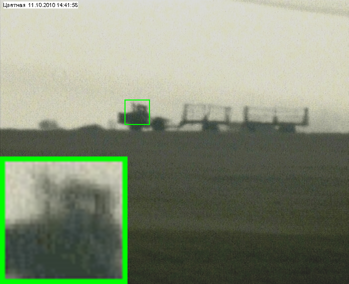
\includegraphics[width=1\textwidth]{imagessupp/resize_br_BM3D_vehicle.png}}
{\footnotesize (b) CBM3D \cite{bm3d,cbm3d}  }
\end{minipage}
\begin{minipage}[t]{0.244\textwidth}
\centering
\raisebox{-0.15cm}{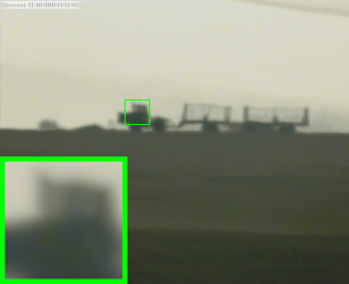
\includegraphics[width=1\textwidth]{imagessupp/resize_br_WNNM_vehicle.png}}
{\footnotesize (c) WNNM \cite{wnnm}   }
\end{minipage} 
\begin{minipage}[t]{0.244\textwidth}
\centering
\raisebox{-0.15cm}{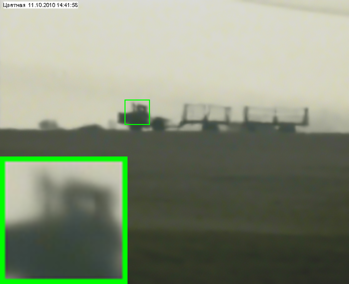
\includegraphics[width=1\textwidth]{imagessupp/resize_br_MLP_vehicle.png}}
{\footnotesize (d) MLP \cite{mlp}  }
\end{minipage}
}\vspace{-2mm}
\subfigure{
\begin{minipage}[t]{0.244\textwidth}
\centering
\raisebox{-0.15cm}{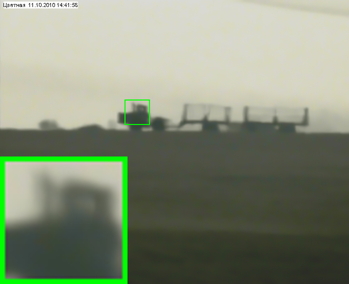
\includegraphics[width=1\textwidth]{imagessupp/resize_br_TRD_vehicle.png}}
{\footnotesize (e) TNRD \cite{chen2015learning}}
\end{minipage}
\begin{minipage}[t]{0.244\textwidth}
\centering
\raisebox{-0.15cm}{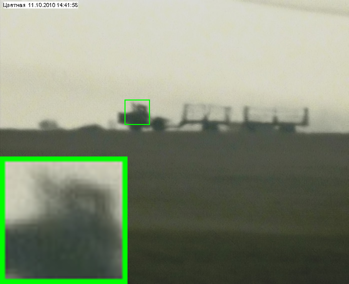
\includegraphics[width=1\textwidth]{imagessupp/resize_br_NI_vehicle.png}}
{\footnotesize (f) NI \cite{neatimage}  }
\end{minipage}
\begin{minipage}[t]{0.244\textwidth}
\centering
\raisebox{-0.15cm}{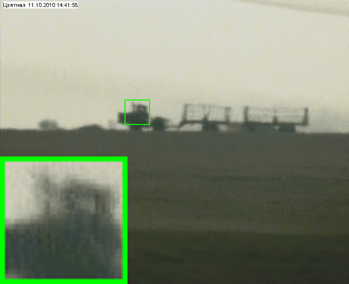
\includegraphics[width=1\textwidth]{imagessupp/resize_br_NC_vehicle.png}}
{\footnotesize (g) NC \cite{ncwebsite,noiseclinic}   }
\end{minipage}
\begin{minipage}[t]{0.244\textwidth}
\centering
\raisebox{-0.15cm}{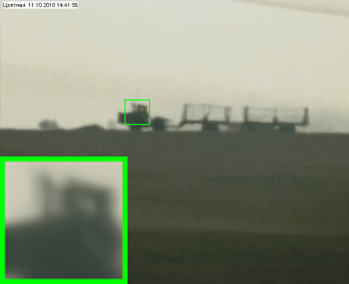
\includegraphics[width=1\textwidth]{imagessupp/resize_br_Guided_vehicle.png}}
{\footnotesize (h) Ours  }
\end{minipage}
}
\caption{Denoised images of the real noisy image ``Vehicle" \cite{ncwebsite} by different methods. The images are better to be zoomed in on screen.}
\label{fig4}
\end{figure}

%------------------------------------------------------------------------------------
%------------------------------------------------------------------------------------
\section{More Results on the 15 Cropped Images Used in \cite{crosschannel2016}}
In this section, we provide more visual comparisons of the proposed method with the state-of-the-art denoising methods on the 15 cropped real noisy images used in \cite{crosschannel2016}. As can be seen from Fiures \ref{fig5}-\ref{fig9}, on most cases, our proposed method achieves better performance than the the competing methods. This validates the effectiveness of our proposed external prior guided internal prior learning framework for real noisy image denoising.

%------------------------------------------------------------------------------------
\begin{figure}[H]\vspace{3mm}
\centering
\subfigure{
\begin{minipage}[t]{0.195\textwidth}
\centering
\raisebox{-0.15cm}{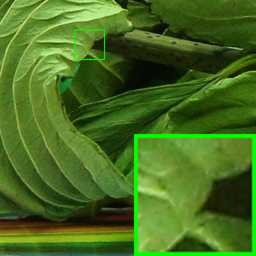
\includegraphics[width=1\textwidth]{imagessupp/resize_br_Noisy_5dmark3_iso3200_2_real.png}}
{\footnotesize (a) Noisy  \cite{crosschannel2016}: 33.88dB }
\end{minipage}
\begin{minipage}[t]{0.195\textwidth}
\centering
\raisebox{-0.15cm}{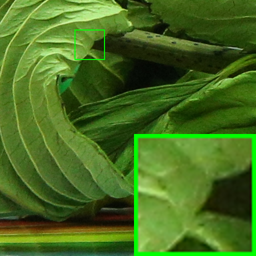
\includegraphics[width=1\textwidth]{imagessupp/resize_br_CBM3D_5dmark3_iso3200_2_real.png}}
{\footnotesize (b) CBM3D \cite{bm3d,cbm3d}: 33.91dB}
\end{minipage}
\begin{minipage}[t]{0.195\textwidth}
\centering
\raisebox{-0.15cm}{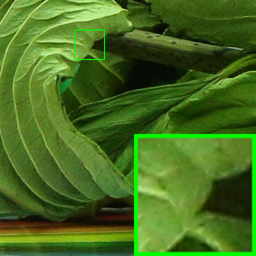
\includegraphics[width=1\textwidth]{imagessupp/resize_br_WNNM_5dmark3_iso3200_2_real.png}}
{\footnotesize (c) WNNM \cite{wnnm}: 33.88dB}
\end{minipage}
\begin{minipage}[t]{0.195\textwidth}
\centering
\raisebox{-0.15cm}{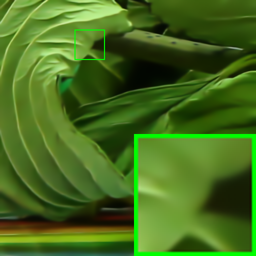
\includegraphics[width=1\textwidth]{imagessupp/resize_br_MLP_5dmark3_iso3200_2_real.png}}
{\footnotesize (d) MLP \cite{mlp}: 33.23dB }
\end{minipage}
\centering
\begin{minipage}[t]{0.195\textwidth}
\raisebox{-0.15cm}{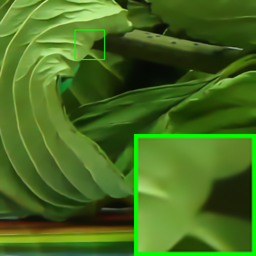
\includegraphics[width=1\textwidth]{imagessupp/resize_br_TRD_5dmark3_iso3200_2_real.png}}
{\footnotesize (e) TNRD \cite{chen2015learning}: 34.33dB  } 
\end{minipage}
}\vspace{-2mm}
\subfigure{
\begin{minipage}[t]{0.195\textwidth}
\centering
\raisebox{-0.15cm}{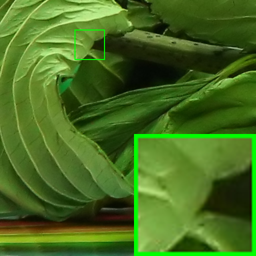
\includegraphics[width=1\textwidth]{imagessupp/resize_br_NI_5dmark3_iso3200_2_real.png}}
{\footnotesize (f) NI \cite{neatimage}: 34.87dB  }
\end{minipage}
\begin{minipage}[t]{0.195\textwidth}
\centering
\raisebox{-0.15cm}{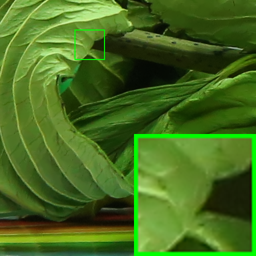
\includegraphics[width=1\textwidth]{imagessupp/resize_br_NC_5dmark3_iso3200_2_real.png}}
{\footnotesize (g) NC \cite{ncwebsite,noiseclinic}: 35.69dB  }
\end{minipage}
\begin{minipage}[t]{0.195\textwidth}
\centering
\raisebox{-0.15cm}{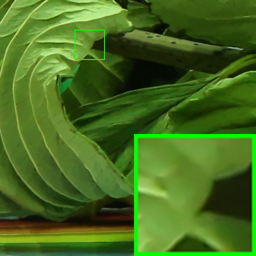
\includegraphics[width=1\textwidth]{imagessupp/resize_br_CCNoise_5dmark3_iso3200_2.png}}
{\footnotesize (h) CC \cite{crosschannel2016}: 35.37dB }
\end{minipage}
\begin{minipage}[t]{0.195\textwidth}
\centering
\raisebox{-0.15cm}{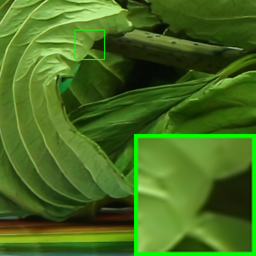
\includegraphics[width=1\textwidth]{imagessupp/resize_br_Guided_5dmark3_iso3200_2_real.png}}
{\footnotesize (i) Ours: \textbf{37.05}dB}
\end{minipage}
\begin{minipage}[t]{0.195\textwidth}
\centering
\raisebox{-0.15cm}{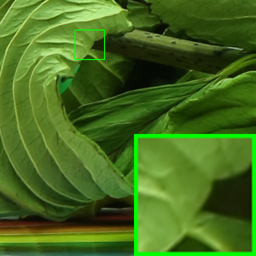
\includegraphics[width=1\textwidth]{imagessupp/resize_br_Mean_5dmark3_iso3200_2_real.png}}
{\footnotesize (j) Mean Image \cite{crosschannel2016}}
\end{minipage}
}
\caption{Denoised images of a region cropped from the real noisy image ``Canon 5D Mark 3 ISO 3200 2" \cite{crosschannel2016} by different methods. The images are better to be zoomed in on screen.}
\label{fig5}
\end{figure}

%------------------------------------------------------------------------------------
\begin{figure}[H]\vspace{1mm}
\centering
\subfigure{
\begin{minipage}[t]{0.195\textwidth}
\centering
\raisebox{-0.15cm}{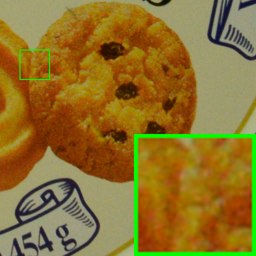
\includegraphics[width=1\textwidth]{imagessupp/resize_br_Noisy_d600_iso3200_2_real.png}}
{\footnotesize (a) Noisy  \cite{crosschannel2016}: 33.77dB }
\end{minipage}
\begin{minipage}[t]{0.195\textwidth}
\centering
\raisebox{-0.15cm}{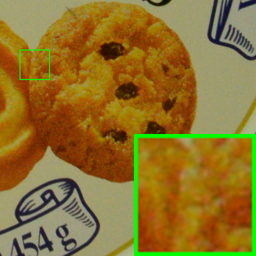
\includegraphics[width=1\textwidth]{imagessupp/resize_br_CBM3D_d600_iso3200_2_real.png}}
{\footnotesize (b) CBM3D \cite{bm3d,cbm3d}: 33.80dB}
\end{minipage}
\begin{minipage}[t]{0.195\textwidth}
\centering
\raisebox{-0.15cm}{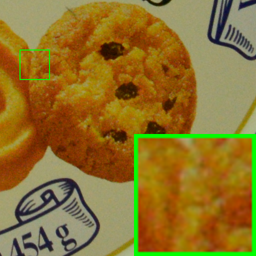
\includegraphics[width=1\textwidth]{imagessupp/resize_br_WNNM_d600_iso3200_2_real.png}}
{\footnotesize (c) WNNM \cite{wnnm}: 33.77dB}
\end{minipage}
\begin{minipage}[t]{0.195\textwidth}
\centering
\raisebox{-0.15cm}{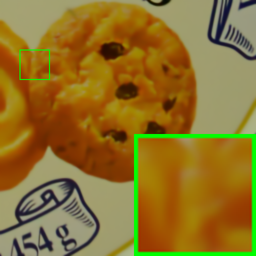
\includegraphics[width=1\textwidth]{imagessupp/resize_br_MLP_d600_iso3200_2_real.png}}
{\footnotesize (d) MLP \cite{mlp}: 34.13dB }
\end{minipage}
\centering
\begin{minipage}[t]{0.195\textwidth}
\raisebox{-0.15cm}{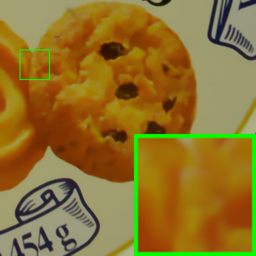
\includegraphics[width=1\textwidth]{imagessupp/resize_br_TRD_d600_iso3200_2_real.png}}
{\footnotesize (e) TNRD \cite{chen2015learning}: 35.32dB  } 
\end{minipage}
}\vspace{-2mm}
\subfigure{
\begin{minipage}[t]{0.195\textwidth}
\centering
\raisebox{-0.15cm}{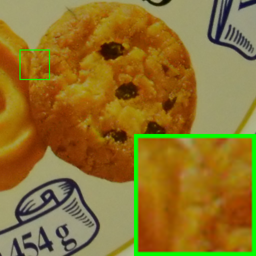
\includegraphics[width=1\textwidth]{imagessupp/resize_br_NI_d600_iso3200_2_real.png}}
{\footnotesize (f) NI \cite{neatimage}: 35.36dB  }
\end{minipage}
\begin{minipage}[t]{0.195\textwidth}
\centering
\raisebox{-0.15cm}{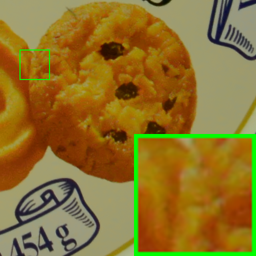
\includegraphics[width=1\textwidth]{imagessupp/resize_br_NC_d600_iso3200_2_real.png}}
{\footnotesize (g) NC \cite{ncwebsite,noiseclinic}: 36.70dB  }
\end{minipage}
\begin{minipage}[t]{0.195\textwidth}
\centering
\raisebox{-0.15cm}{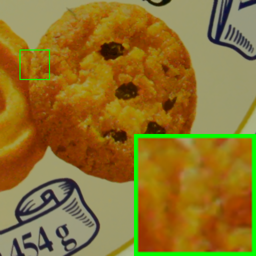
\includegraphics[width=1\textwidth]{imagessupp/resize_br_CCNoise_d600_iso3200_2.png}}
{\footnotesize (h) CC \cite{crosschannel2016}: 35.95dB }
\end{minipage}
\begin{minipage}[t]{0.195\textwidth}
\centering
\raisebox{-0.15cm}{\includegraphics[width=1\textwidth]{imagessupp/resize_br_Guided_d600_iso3200_2_real.png}}
{\footnotesize (i) Ours: \textbf{36.31}dB}
\end{minipage}
\begin{minipage}[t]{0.195\textwidth}
\centering
\raisebox{-0.15cm}{\includegraphics[width=1\textwidth]{imagessupp/resize_br_Mean_d600_iso3200_2_real.png}}
{\footnotesize (j) Mean Image \cite{crosschannel2016}}
\end{minipage}
}
\caption{Denoised images of a region cropped from the real noisy image ``Canon 5D Mark 3 ISO 3200 2" \cite{crosschannel2016} by different methods. The images are better to be zoomed in on screen.}
\label{fig6}
\end{figure}


%------------------------------------------------------------------------------------
\begin{figure}[H]\vspace{1mm}
\centering
\subfigure{
\begin{minipage}[t]{0.195\textwidth}
\centering
\raisebox{-0.15cm}{\includegraphics[width=1\textwidth]{imagessupp/resize_br_Noisy_d800_iso1600_2_real.png}}
{\footnotesize (a) Noisy  \cite{crosschannel2016}: 35.71dB }
\end{minipage}
\begin{minipage}[t]{0.195\textwidth}
\centering
\raisebox{-0.15cm}{\includegraphics[width=1\textwidth]{imagessupp/resize_br_CBM3D_d800_iso1600_2_real.png}}
{\footnotesize (b) CBM3D \cite{bm3d,cbm3d}: 35.73dB}
\end{minipage}
\begin{minipage}[t]{0.195\textwidth}
\centering
\raisebox{-0.15cm}{\includegraphics[width=1\textwidth]{imagessupp/resize_br_WNNM_d800_iso1600_2_real.png}}
{\footnotesize (c) WNNM \cite{wnnm}: 35.71dB}
\end{minipage}
\begin{minipage}[t]{0.195\textwidth}
\centering
\raisebox{-0.15cm}{\includegraphics[width=1\textwidth]{imagessupp/resize_br_MLP_d800_iso1600_2_real.png}}
{\footnotesize (d) MLP \cite{mlp}: 35.87dB }
\end{minipage}
\centering
\begin{minipage}[t]{0.195\textwidth}
\raisebox{-0.15cm}{\includegraphics[width=1\textwidth]{imagessupp/resize_br_TRD_d800_iso1600_2_real.png}}
{\footnotesize (e) TNRD \cite{chen2015learning}: 38.61dB  } 
\end{minipage}
}\vspace{-2mm}
\subfigure{
\begin{minipage}[t]{0.195\textwidth}
\centering
\raisebox{-0.15cm}{\includegraphics[width=1\textwidth]{imagessupp/resize_br_NI_d800_iso1600_2_real.png}}
{\footnotesize (f) NI \cite{neatimage}: 38.57dB  }
\end{minipage}
\begin{minipage}[t]{0.195\textwidth}
\centering
\raisebox{-0.15cm}{\includegraphics[width=1\textwidth]{imagessupp/resize_br_NC_d800_iso1600_2_real.png}}
{\footnotesize (g) NC \cite{ncwebsite,noiseclinic}: 39.05dB  }
\end{minipage}
\begin{minipage}[t]{0.195\textwidth}
\centering
\raisebox{-0.15cm}{\includegraphics[width=1\textwidth]{imagessupp/resize_br_CCNoise_d800_iso1600_2.png}}
{\footnotesize (h) CC \cite{crosschannel2016}: 40.36dB }
\end{minipage}
\begin{minipage}[t]{0.195\textwidth}
\centering
\raisebox{-0.15cm}{\includegraphics[width=1\textwidth]{imagessupp/resize_br_Guided_d800_iso1600_2_real.png}}
{\footnotesize (i) Ours: \textbf{40.92}dB}
\end{minipage}
\begin{minipage}[t]{0.195\textwidth}
\centering
\raisebox{-0.15cm}{\includegraphics[width=1\textwidth]{imagessupp/resize_br_Mean_d800_iso1600_2_real.png}}
{\footnotesize (j) Mean Image \cite{crosschannel2016}}
\end{minipage}
}
\caption{Denoised images of a region cropped from the real noisy image ``Nikon D800 ISO 1600 2" \cite{crosschannel2016} by different methods. The images are better to be zoomed in on screen.}
\label{fig7}
\end{figure}


%------------------------------------------------------------------------------------
\begin{figure}[H]\vspace{1mm}
\centering
\subfigure{
\begin{minipage}[t]{0.195\textwidth}
\centering
\raisebox{-0.15cm}{\includegraphics[width=1\textwidth]{imagessupp/resize_br_Noisy_d800_iso3200_2_real.png}}
{\footnotesize (a) Noisy  \cite{crosschannel2016}: 32.89dB }
\end{minipage}
\begin{minipage}[t]{0.195\textwidth}
\centering
\raisebox{-0.15cm}{\includegraphics[width=1\textwidth]{imagessupp/resize_br_CBM3D_d800_iso3200_2_real.png}}
{\footnotesize (b) CBM3D \cite{bm3d,cbm3d}: 32.91dB}
\end{minipage}
\begin{minipage}[t]{0.195\textwidth}
\centering
\raisebox{-0.15cm}{\includegraphics[width=1\textwidth]{imagessupp/resize_br_WNNM_d800_iso3200_2_real.png}}
{\footnotesize (c) WNNM \cite{wnnm}: 32.94dB}
\end{minipage}
\begin{minipage}[t]{0.195\textwidth}
\centering
\raisebox{-0.15cm}{\includegraphics[width=1\textwidth]{imagessupp/resize_br_MLP_d800_iso3200_2_real.png}}
{\footnotesize (d) MLP \cite{mlp}: 34.87dB }
\end{minipage}
\centering
\begin{minipage}[t]{0.195\textwidth}
\raisebox{-0.15cm}{\includegraphics[width=1\textwidth]{imagessupp/resize_br_TRD_d800_iso3200_2_real.png}}
{\footnotesize (e) TNRD \cite{chen2015learning}: 35.74dB  } 
\end{minipage}
}\vspace{-2mm}
\subfigure{
\begin{minipage}[t]{0.195\textwidth}
\centering
\raisebox{-0.15cm}{\includegraphics[width=1\textwidth]{imagessupp/resize_br_NI_d800_iso3200_2_real.png}}
{\footnotesize (f) NI \cite{neatimage}: 35.09dB  }
\end{minipage}
\begin{minipage}[t]{0.195\textwidth}
\centering
\raisebox{-0.15cm}{\includegraphics[width=1\textwidth]{imagessupp/resize_br_NC_d800_iso3200_2_real.png}}
{\footnotesize (g) NC \cite{ncwebsite,noiseclinic}: 35.72dB  }
\end{minipage}
\begin{minipage}[t]{0.195\textwidth}
\centering
\raisebox{-0.15cm}{\includegraphics[width=1\textwidth]{imagessupp/resize_br_CCNoise_d800_iso3200_2.png}}
{\footnotesize (h) CC \cite{crosschannel2016}: 36.75dB }
\end{minipage}
\begin{minipage}[t]{0.195\textwidth}
\centering
\raisebox{-0.15cm}{\includegraphics[width=1\textwidth]{imagessupp/resize_br_Guided_d800_iso3200_2_real.png}}
{\footnotesize (i) Ours: \textbf{37.07}dB}
\end{minipage}
\begin{minipage}[t]{0.195\textwidth}
\centering
\raisebox{-0.15cm}{\includegraphics[width=1\textwidth]{imagessupp/resize_br_Mean_d800_iso3200_2_real.png}}
{\footnotesize (j) Mean Image \cite{crosschannel2016}}
\end{minipage}
}
\caption{Denoised images of a region cropped from the real noisy image ``Nikon D800 ISO 3200 2" \cite{crosschannel2016} by different methods. The images are better to be zoomed in on screen.}
\label{fig8}
\end{figure}

%------------------------------------------------------------------------------------
\begin{figure}[H]\vspace{1mm}
\centering
\subfigure{
\begin{minipage}[t]{0.195\textwidth}
\centering
\raisebox{-0.15cm}{\includegraphics[width=1\textwidth]{imagessupp/resize_br_Noisy_d800_iso6400_2_real.png}}
{\footnotesize (a) Noisy  \cite{crosschannel2016}: 29.97dB }
\end{minipage}
\begin{minipage}[t]{0.195\textwidth}
\centering
\raisebox{-0.15cm}{\includegraphics[width=1\textwidth]{imagessupp/resize_br_CBM3D_d800_iso6400_2_real.png}}
{\footnotesize (b) CBM3D \cite{bm3d,cbm3d}: 29.99dB}
\end{minipage}
\begin{minipage}[t]{0.195\textwidth}
\centering
\raisebox{-0.15cm}{\includegraphics[width=1\textwidth]{imagessupp/resize_br_WNNM_d800_iso6400_2_real.png}}
{\footnotesize (c) WNNM \cite{wnnm}: 329.97dB}
\end{minipage}
\begin{minipage}[t]{0.195\textwidth}
\centering
\raisebox{-0.15cm}{\includegraphics[width=1\textwidth]{imagessupp/resize_br_MLP_d800_iso6400_2_real.png}}
{\footnotesize (d) MLP \cite{mlp}: 31.55dB }
\end{minipage}
\centering
\begin{minipage}[t]{0.195\textwidth}
\raisebox{-0.15cm}{\includegraphics[width=1\textwidth]{imagessupp/resize_br_TRD_d800_iso6400_2_real.png}}
{\footnotesize (e) TNRD \cite{chen2015learning}: 32.37dB  } 
\end{minipage}
}\vspace{-2mm}
\subfigure{
\begin{minipage}[t]{0.195\textwidth}
\centering
\raisebox{-0.15cm}{\includegraphics[width=1\textwidth]{imagessupp/resize_br_NI_d800_iso6400_2_real.png}}
{\footnotesize (f) NI \cite{neatimage}: 31.38dB  }
\end{minipage}
\begin{minipage}[t]{0.195\textwidth}
\centering
\raisebox{-0.15cm}{\includegraphics[width=1\textwidth]{imagessupp/resize_br_NC_d800_iso6400_2_real.png}}
{\footnotesize (g) NC \cite{ncwebsite,noiseclinic}: 32.79dB  }
\end{minipage}
\begin{minipage}[t]{0.195\textwidth}
\centering
\raisebox{-0.15cm}{\includegraphics[width=1\textwidth]{imagessupp/resize_br_CCNoise_d800_iso6400_2.png}}
{\footnotesize (h) CC \cite{crosschannel2016}: 33.21dB }
\end{minipage}
\begin{minipage}[t]{0.195\textwidth}
\centering
\raisebox{-0.15cm}{\includegraphics[width=1\textwidth]{imagessupp/resize_br_Guided_d800_iso6400_2_real.png}}
{\footnotesize (i) Ours: \textbf{33.43}dB}
\end{minipage}
\begin{minipage}[t]{0.195\textwidth}
\centering
\raisebox{-0.15cm}{\includegraphics[width=1\textwidth]{imagessupp/resize_br_Mean_d800_iso6400_2_real.png}}
{\footnotesize (j) Mean Image \cite{crosschannel2016}}
\end{minipage}
}
\caption{Denoised images of a region cropped from the real noisy image ``Nikon D800 ISO 6400 2" \cite{crosschannel2016} by different methods. The images are better to be zoomed in on screen.}
\label{fig9}
\end{figure}

\section{More Results on the 60 Cropped Images in \cite{crosschannel2016}}
In this section, we provide more visual comparisons of the proposed method with the state-of-the-art denoising methods on the 60 cropped real noisy images we cropped fromfrom \cite{crosschannel2016}. As can be seen from Fiures \ref{fig10}-\ref{fig15}, on most cases, our proposed method achieves better performance than the the competing methods. This validates the effectiveness of our proposed external prior guided internal prior learning framework for real noisy image denoising.

%------------------------------------------------------------------------------------
\begin{figure}[H]\vspace{1mm}
\centering
\subfigure{
\begin{minipage}[t]{0.195\textwidth}
\centering
\raisebox{-0.15cm}{\includegraphics[width=1\textwidth]{imagessupp/resize_br_Noisy_CC_Noisy_Canon_EOS_5D_Mark3_ISO_3200_C1_47.png}}
{\footnotesize (a) Noisy \cite{crosschannel2016}: 36.15dB }
\end{minipage}
\begin{minipage}[t]{0.195\textwidth}
\centering
\raisebox{-0.15cm}{\includegraphics[width=1\textwidth]{imagessupp/resize_br_CBM3D_CC_Noisy_Canon_EOS_5D_Mark3_ISO_3200_C1_47.png}}
{\footnotesize (b) CBM3D \cite{bm3d,cbm3d}: 36.20dB  }
\end{minipage}
\begin{minipage}[t]{0.195\textwidth}
\centering
\raisebox{-0.15cm}{\includegraphics[width=1\textwidth]{imagessupp/resize_br_WNNM_CC_Noisy_Canon_EOS_5D_Mark3_ISO_3200_C1_47.png}}
{\footnotesize (c) WNNM \cite{wnnm}: 36.15dB  }
\end{minipage}
\begin{minipage}[t]{0.195\textwidth}
\centering
\raisebox{-0.15cm}{\includegraphics[width=1\textwidth]{imagessupp/resize_br_MLP_CC_Noisy_Canon_EOS_5D_Mark3_ISO_3200_C1_47.png}}
{\footnotesize (d) MLP \cite{mlp}: 34.10dB }
\end{minipage}
\begin{minipage}[t]{0.195\textwidth}
\centering
\raisebox{-0.15cm}{\includegraphics[width=1\textwidth]{imagessupp/resize_br_CSF_CC_Noisy_Canon_EOS_5D_Mark3_ISO_3200_C1_47.png}}
{\footnotesize (e) CSF \cite{csf}: 35.47dB }
\end{minipage}
}\vspace{-3mm}
\subfigure{
\begin{minipage}[t]{0.195\textwidth}
\centering
\raisebox{-0.15cm}{\includegraphics[width=1\textwidth]{imagessupp/resize_br_TRD_CC_Noisy_Canon_EOS_5D_Mark3_ISO_3200_C1_47.png}}
{\footnotesize (f) TNRD \cite{chen2015learning}: 35.94dB   }
\end{minipage}
\begin{minipage}[t]{0.195\textwidth}
\centering
\raisebox{-0.15cm}{\includegraphics[width=1\textwidth]{imagessupp/resize_br_NI_CC_Noisy_Canon_EOS_5D_Mark3_ISO_3200_C1_47.png}}
{\footnotesize (g) NI \cite{neatimage}: 36.72dB  }
\end{minipage}
\begin{minipage}[t]{0.195\textwidth}
\centering
\raisebox{-0.15cm}{\includegraphics[width=1\textwidth]{imagessupp/resize_br_NC_CC_Noisy_Canon_EOS_5D_Mark3_ISO_3200_C1_47.png}}
{\footnotesize (h) NC \cite{ncwebsite,noiseclinic}: 37.45dB   }
\end{minipage}
\begin{minipage}[t]{0.195\textwidth}
\centering
\raisebox{-0.15cm}{\includegraphics[width=1\textwidth]{imagessupp/resize_br_Guided_CC_Noisy_Canon_EOS_5D_Mark3_ISO_3200_C1_47.png}}
{\footnotesize (i) Ours: \textbf{38.09}dB  }
\end{minipage}
\begin{minipage}[t]{0.195\textwidth}
\centering
\raisebox{-0.15cm}{\includegraphics[width=1\textwidth]{imagessupp/resize_br_Mean_CC_Noisy_Canon_EOS_5D_Mark3_ISO_3200_C1_47.png}}
{\footnotesize (j) Mean Image \cite{crosschannel2016} }
\end{minipage}
}
\caption{Denoised imagessupp of a region cropped from the real noisy image ``Canon EOS 5D Mark3 ISO 3200 C1" \cite{crosschannel2016} by different methods. The images are better viewed by zooming in on screen.} 
\label{fig10}
\end{figure}

%------------------------------------------------------------------------------------
\begin{figure}[H]\vspace{1mm}
\centering
\subfigure{
\begin{minipage}[t]{0.195\textwidth}
\centering
\raisebox{-0.15cm}{\includegraphics[width=1\textwidth]{imagessupp/resize_br_Noisy_CC_Noisy_Canon_EOS_5D_Mark3_ISO_3200_C2_44.png}}
{\footnotesize (a) Noisy \cite{crosschannel2016}: 35.97dB }
\end{minipage}
\begin{minipage}[t]{0.195\textwidth}
\centering
\raisebox{-0.15cm}{\includegraphics[width=1\textwidth]{imagessupp/resize_br_CBM3D_CC_Noisy_Canon_EOS_5D_Mark3_ISO_3200_C2_44.png}}
{\footnotesize (b) CBM3D \cite{bm3d,cbm3d}: 35.99dB  }
\end{minipage}
\begin{minipage}[t]{0.195\textwidth}
\centering
\raisebox{-0.15cm}{\includegraphics[width=1\textwidth]{imagessupp/resize_br_WNNM_CC_Noisy_Canon_EOS_5D_Mark3_ISO_3200_C2_44.png}}
{\footnotesize (c) WNNM \cite{wnnm}: 36.00dB  }
\end{minipage}
\begin{minipage}[t]{0.195\textwidth}
\centering
\raisebox{-0.15cm}{\includegraphics[width=1\textwidth]{imagessupp/resize_br_MLP_CC_Noisy_Canon_EOS_5D_Mark3_ISO_3200_C2_44.png}}
{\footnotesize (d) MLP \cite{mlp}: 36.84dB }
\end{minipage}
\begin{minipage}[t]{0.195\textwidth}
\centering
\raisebox{-0.15cm}{\includegraphics[width=1\textwidth]{imagessupp/resize_br_CSF_CC_Noisy_Canon_EOS_5D_Mark3_ISO_3200_C2_44.png}}
{\footnotesize (e) CSF \cite{csf}: 37.73dB }
\end{minipage}
}\vspace{-3mm}
\subfigure{
\begin{minipage}[t]{0.195\textwidth}
\centering
\raisebox{-0.15cm}{\includegraphics[width=1\textwidth]{imagessupp/resize_br_TRD_CC_Noisy_Canon_EOS_5D_Mark3_ISO_3200_C2_44.png}}
{\footnotesize (f) TNRD \cite{chen2015learning}: 38.31dB   }
\end{minipage}
\begin{minipage}[t]{0.195\textwidth}
\centering
\raisebox{-0.15cm}{\includegraphics[width=1\textwidth]{imagessupp/resize_br_NI_CC_Noisy_Canon_EOS_5D_Mark3_ISO_3200_C2_44.png}}
{\footnotesize (g) NI \cite{neatimage}: 37.45dB  }
\end{minipage}
\begin{minipage}[t]{0.195\textwidth}
\centering
\raisebox{-0.15cm}{\includegraphics[width=1\textwidth]{imagessupp/resize_br_NC_CC_Noisy_Canon_EOS_5D_Mark3_ISO_3200_C2_44.png}}
{\footnotesize (h) NC \cite{ncwebsite,noiseclinic}: 38.01dB   }
\end{minipage}
\begin{minipage}[t]{0.195\textwidth}
\centering
\raisebox{-0.15cm}{\includegraphics[width=1\textwidth]{imagessupp/resize_br_Guided_CC_Noisy_Canon_EOS_5D_Mark3_ISO_3200_C2_44.png}}
{\footnotesize (i) Ours: \textbf{40.07}dB  }
\end{minipage}
\begin{minipage}[t]{0.195\textwidth}
\centering
\raisebox{-0.15cm}{\includegraphics[width=1\textwidth]{imagessupp/resize_br_Mean_CC_Noisy_Canon_EOS_5D_Mark3_ISO_3200_C2_44.png}}
{\footnotesize (j) Mean Image \cite{crosschannel2016} }
\end{minipage}
}
\caption{Denoised imagessupp of a region cropped from the real noisy image ``Canon EOS 5D Mark3 ISO 3200 C2" \cite{crosschannel2016} by different methods. The images are better viewed by zooming in on screen.} 
\label{fig11}
\end{figure}


%------------------------------------------------------------------------------------
\begin{figure}[H]\vspace{1mm}
\centering
\subfigure{
\begin{minipage}[t]{0.195\textwidth}
\centering
\raisebox{-0.15cm}{\includegraphics[width=1\textwidth]{imagessupp/resize_br_Noisy_CC_Noisy_Canon_EOS_5D_Mark3_ISO_3200_C3_26.png}}
{\footnotesize (a) Noisy \cite{crosschannel2016}: 34.40dB }
\end{minipage}
\begin{minipage}[t]{0.195\textwidth}
\centering
\raisebox{-0.15cm}{\includegraphics[width=1\textwidth]{imagessupp/resize_br_CBM3D_CC_Noisy_Canon_EOS_5D_Mark3_ISO_3200_C3_26.png}}
{\footnotesize (b) CBM3D \cite{bm3d,cbm3d}: 34.40dB  }
\end{minipage}
\begin{minipage}[t]{0.195\textwidth}
\centering
\raisebox{-0.15cm}{\includegraphics[width=1\textwidth]{imagessupp/resize_br_WNNM_CC_Noisy_Canon_EOS_5D_Mark3_ISO_3200_C3_26.png}}
{\footnotesize (c) WNNM \cite{wnnm}: 34.44dB  }
\end{minipage}
\begin{minipage}[t]{0.195\textwidth}
\centering
\raisebox{-0.15cm}{\includegraphics[width=1\textwidth]{imagessupp/resize_br_MLP_CC_Noisy_Canon_EOS_5D_Mark3_ISO_3200_C3_26.png}}
{\footnotesize (d) MLP \cite{mlp}: 33.02dB }
\end{minipage}
\begin{minipage}[t]{0.195\textwidth}
\centering
\raisebox{-0.15cm}{\includegraphics[width=1\textwidth]{imagessupp/resize_br_CSF_CC_Noisy_Canon_EOS_5D_Mark3_ISO_3200_C3_26.png}}
{\footnotesize (e) CSF \cite{csf}: 33.71dB }
\end{minipage}
}\vspace{-3mm}
\subfigure{
\begin{minipage}[t]{0.195\textwidth}
\centering
\raisebox{-0.15cm}{\includegraphics[width=1\textwidth]{imagessupp/resize_br_TRD_CC_Noisy_Canon_EOS_5D_Mark3_ISO_3200_C3_26.png}}
{\footnotesize (f) TNRD \cite{chen2015learning}: 34.03dB   }
\end{minipage}
\begin{minipage}[t]{0.195\textwidth}
\centering
\raisebox{-0.15cm}{\includegraphics[width=1\textwidth]{imagessupp/resize_br_NI_CC_Noisy_Canon_EOS_5D_Mark3_ISO_3200_C3_26.png}}
{\footnotesize (g) NI \cite{neatimage}: 36.11dB  }
\end{minipage}
\begin{minipage}[t]{0.195\textwidth}
\centering
\raisebox{-0.15cm}{\includegraphics[width=1\textwidth]{imagessupp/resize_br_NC_CC_Noisy_Canon_EOS_5D_Mark3_ISO_3200_C3_26.png}}
{\footnotesize (h) NC \cite{ncwebsite,noiseclinic}: 36.51dB   }
\end{minipage}
\begin{minipage}[t]{0.195\textwidth}
\centering
\raisebox{-0.15cm}{\includegraphics[width=1\textwidth]{imagessupp/resize_br_Guided_CC_Noisy_Canon_EOS_5D_Mark3_ISO_3200_C3_26.png}}
{\footnotesize (i) Ours: \textbf{38.32}dB  }
\end{minipage}
\begin{minipage}[t]{0.195\textwidth}
\centering
\raisebox{-0.15cm}{\includegraphics[width=1\textwidth]{imagessupp/resize_br_Mean_CC_Noisy_Canon_EOS_5D_Mark3_ISO_3200_C3_26.png}}
{\footnotesize (j) Mean Image \cite{crosschannel2016} }
\end{minipage}
}
\caption{Denoised imagessupp of a region cropped from the real noisy image ``Canon EOS 5D Mark3 ISO 3200 C3" \cite{crosschannel2016} by different methods. The images are better viewed by zooming in on screen.} 
\label{fig12}
\end{figure}

%------------------------------------------------------------------------------------
\begin{figure}[H]\vspace{1mm}
\centering
\subfigure{
\begin{minipage}[t]{0.196\textwidth}
\centering
\raisebox{-0.15cm}{\includegraphics[width=1\textwidth]{imagessupp/resize_br_Noisy_CC_Noisy_Nikon_D600_ISO_3200_C1_96.png}}
{\footnotesize (a) Noisy \cite{crosschannel2016}: 35.89dB }
\end{minipage}
\begin{minipage}[t]{0.196\textwidth}
\centering
\raisebox{-0.15cm}{\includegraphics[width=1\textwidth]{imagessupp/resize_br_CBM3D_CC_Noisy_Nikon_D600_ISO_3200_C1_96.png}}
{\footnotesize (b) CBM3D \cite{bm3d,cbm3d}: 35.92dB  }
\end{minipage}
\begin{minipage}[t]{0.196\textwidth}
\centering
\raisebox{-0.15cm}{\includegraphics[width=1\textwidth]{imagessupp/resize_br_WNNM_CC_Noisy_Nikon_D600_ISO_3200_C1_96.png}}
{\footnotesize (c) WNNM \cite{wnnm}: 35.89dB  }
\end{minipage}
\begin{minipage}[t]{0.196\textwidth}
\centering
\raisebox{-0.15cm}{\includegraphics[width=1\textwidth]{imagessupp/resize_br_MLP_CC_Noisy_Nikon_D600_ISO_3200_C1_96.png}}
{\footnotesize (d) MLP \cite{mlp}: 34.82dB }
\end{minipage}
\begin{minipage}[t]{0.196\textwidth}
\centering
\raisebox{-0.15cm}{\includegraphics[width=1\textwidth]{imagessupp/resize_br_CSF_CC_Noisy_Nikon_D600_ISO_3200_C1_96.png}}
{\footnotesize (e) CSF \cite{csf}: 36.85dB }
\end{minipage}
}\vspace{-3mm}
\subfigure{
\begin{minipage}[t]{0.196\textwidth}
\centering
\raisebox{-0.15cm}{\includegraphics[width=1\textwidth]{imagessupp/resize_br_TRD_CC_Noisy_Nikon_D600_ISO_3200_C1_96.png}}
{\footnotesize (f) TNRD \cite{chen2015learning}: 37.35dB   }
\end{minipage}
\begin{minipage}[t]{0.196\textwidth}
\centering
\raisebox{-0.15cm}{\includegraphics[width=1\textwidth]{imagessupp/resize_br_NI_CC_Noisy_Nikon_D600_ISO_3200_C1_96.png}}
{\footnotesize (g) NI \cite{neatimage}: 37.37dB  }
\end{minipage}
\begin{minipage}[t]{0.196\textwidth}
\centering
\raisebox{-0.15cm}{\includegraphics[width=1\textwidth]{imagessupp/resize_br_NC_CC_Noisy_Nikon_D600_ISO_3200_C1_96.png}}
{\footnotesize (h) NC \cite{ncwebsite,noiseclinic}: 38.48dB   }
\end{minipage}
\begin{minipage}[t]{0.196\textwidth}
\centering
\raisebox{-0.15cm}{\includegraphics[width=1\textwidth]{imagessupp/resize_br_Guided_CC_Noisy_Nikon_D600_ISO_3200_C1_96.png}}
{\footnotesize (i) Ours: \textbf{39.66}dB  }
\end{minipage}
\begin{minipage}[t]{0.196\textwidth}
\centering
\raisebox{-0.15cm}{\includegraphics[width=1\textwidth]{imagessupp/resize_br_Mean_CC_Noisy_Nikon_D600_ISO_3200_C1_96.png}}
{\footnotesize (j) Mean Image \cite{crosschannel2016} }
\end{minipage}
}
\caption{Denoised imagessupp of a region cropped from the real noisy image ``Nikon D600 ISO 3200 C1" \cite{crosschannel2016} by different methods. The images are better viewed by zooming in on screen.} 
\label{fig13}
\end{figure}

%------------------------------------------------------------------------------------
\begin{figure}[H]\vspace{1mm}
\centering
\subfigure{
\begin{minipage}[t]{0.196\textwidth}
\centering
\raisebox{-0.15cm}{\includegraphics[width=1\textwidth]{imagessupp/resize_br_Noisy_CC_Noisy_Nikon_D600_ISO_3200_C2_67.png}}
{\footnotesize (a) Noisy \cite{crosschannel2016}: 36.39dB }
\end{minipage}
\begin{minipage}[t]{0.196\textwidth}
\centering
\raisebox{-0.15cm}{\includegraphics[width=1\textwidth]{imagessupp/resize_br_CBM3D_CC_Noisy_Nikon_D600_ISO_3200_C2_67.png}}
{\footnotesize (b) CBM3D \cite{bm3d,cbm3d}: 36.41dB  }
\end{minipage}
\begin{minipage}[t]{0.196\textwidth}
\centering
\raisebox{-0.15cm}{\includegraphics[width=1\textwidth]{imagessupp/resize_br_WNNM_CC_Noisy_Nikon_D600_ISO_3200_C2_67.png}}
{\footnotesize (c) WNNM \cite{wnnm}: 36.39dB  }
\end{minipage}
\begin{minipage}[t]{0.196\textwidth}
\centering
\raisebox{-0.15cm}{\includegraphics[width=1\textwidth]{imagessupp/resize_br_MLP_CC_Noisy_Nikon_D600_ISO_3200_C2_67.png}}
{\footnotesize (d) MLP \cite{mlp}: 35.62dB }
\end{minipage}
\begin{minipage}[t]{0.196\textwidth}
\centering
\raisebox{-0.15cm}{\includegraphics[width=1\textwidth]{imagessupp/resize_br_CSF_CC_Noisy_Nikon_D600_ISO_3200_C2_67.png}}
{\footnotesize (e) CSF \cite{csf}: 38.16dB }
\end{minipage}
}\vspace{-3mm}
\subfigure{
\begin{minipage}[t]{0.196\textwidth}
\centering
\raisebox{-0.15cm}{\includegraphics[width=1\textwidth]{imagessupp/resize_br_TRD_CC_Noisy_Nikon_D600_ISO_3200_C2_67.png}}
{\footnotesize (f) TNRD \cite{chen2015learning}: 38.26dB   }
\end{minipage}
\begin{minipage}[t]{0.196\textwidth}
\centering
\raisebox{-0.15cm}{\includegraphics[width=1\textwidth]{imagessupp/resize_br_NI_CC_Noisy_Nikon_D600_ISO_3200_C2_67.png}}
{\footnotesize (g) NI \cite{neatimage}: 39.84dB  }
\end{minipage}
\begin{minipage}[t]{0.196\textwidth}
\centering
\raisebox{-0.15cm}{\includegraphics[width=1\textwidth]{imagessupp/resize_br_NC_CC_Noisy_Nikon_D600_ISO_3200_C2_67.png}}
{\footnotesize (h) NC \cite{ncwebsite,noiseclinic}: 39.33dB   }
\end{minipage}
\begin{minipage}[t]{0.196\textwidth}
\centering
\raisebox{-0.15cm}{\includegraphics[width=1\textwidth]{imagessupp/resize_br_Guided_CC_Noisy_Nikon_D600_ISO_3200_C2_67.png}}
{\footnotesize (i) Ours: \textbf{40.36}dB  }
\end{minipage}
\begin{minipage}[t]{0.196\textwidth}
\centering
\raisebox{-0.15cm}{\includegraphics[width=1\textwidth]{imagessupp/resize_br_Mean_CC_Noisy_Nikon_D600_ISO_3200_C2_67.png}}
{\footnotesize (j) Mean Image \cite{crosschannel2016} }
\end{minipage}
}
\caption{Denoised imagessupp of a region cropped from the real noisy image ``Nikon D600 ISO 3200 C2" \cite{crosschannel2016} by different methods. The images are better viewed by zooming in on screen.} 
\label{fig14}
\end{figure}

%------------------------------------------------------------------------------------
\begin{figure}[H]\vspace{1mm}
\centering
\subfigure{
\begin{minipage}[t]{0.196\textwidth}
\centering
\raisebox{-0.15cm}{\includegraphics[width=1\textwidth]{imagessupp/resize_br_Noisy_CC_Noisy_Nikon_D800_ISO_1600_B2_109.png}}
{\footnotesize (a) Noisy \cite{crosschannel2016}: 35.21dB }
\end{minipage}
\begin{minipage}[t]{0.196\textwidth}
\centering
\raisebox{-0.15cm}{\includegraphics[width=1\textwidth]{imagessupp/resize_br_CBM3D_CC_Noisy_Nikon_D800_ISO_1600_B2_109.png}}
{\footnotesize (b) CBM3D \cite{bm3d,cbm3d}: 35.25dB  }
\end{minipage}
\begin{minipage}[t]{0.196\textwidth}
\centering
\raisebox{-0.15cm}{\includegraphics[width=1\textwidth]{imagessupp/resize_br_WNNM_CC_Noisy_Nikon_D800_ISO_1600_B2_109.png}}
{\footnotesize (c) WNNM \cite{wnnm}: 35.21dB  }
\end{minipage}
\begin{minipage}[t]{0.196\textwidth}
\centering
\raisebox{-0.15cm}{\includegraphics[width=1\textwidth]{imagessupp/resize_br_MLP_CC_Noisy_Nikon_D800_ISO_1600_B2_109.png}}
{\footnotesize (d) MLP \cite{mlp}: 37.18dB }
\end{minipage}
\begin{minipage}[t]{0.196\textwidth}
\centering
\raisebox{-0.15cm}{\includegraphics[width=1\textwidth]{imagessupp/resize_br_CSF_CC_Noisy_Nikon_D800_ISO_1600_B2_109.png}}
{\footnotesize (e) CSF \cite{csf}: 38.10dB }
\end{minipage}
}\vspace{-3mm}
\subfigure{
\begin{minipage}[t]{0.196\textwidth}
\centering
\raisebox{-0.15cm}{\includegraphics[width=1\textwidth]{imagessupp/resize_br_TRD_CC_Noisy_Nikon_D800_ISO_1600_B2_109.png}}
{\footnotesize (f) TNRD \cite{chen2015learning}: 38.62dB   }
\end{minipage}
\begin{minipage}[t]{0.196\textwidth}
\centering
\raisebox{-0.15cm}{\includegraphics[width=1\textwidth]{imagessupp/resize_br_NI_CC_Noisy_Nikon_D800_ISO_1600_B2_109.png}}
{\footnotesize (g) NI \cite{neatimage}: 37.41dB  }
\end{minipage}
\begin{minipage}[t]{0.196\textwidth}
\centering
\raisebox{-0.15cm}{\includegraphics[width=1\textwidth]{imagessupp/resize_br_NC_CC_Noisy_Nikon_D800_ISO_1600_B2_109.png}}
{\footnotesize (h) NC \cite{ncwebsite,noiseclinic}: 39.53dB   }
\end{minipage}
\begin{minipage}[t]{0.196\textwidth}
\centering
\raisebox{-0.15cm}{\includegraphics[width=1\textwidth]{imagessupp/resize_br_Guided_CC_Noisy_Nikon_D800_ISO_1600_B2_109.png}}
{\footnotesize (i) Ours: \textbf{39.87}dB  }
\end{minipage}
\begin{minipage}[t]{0.196\textwidth}
\centering
\raisebox{-0.15cm}{\includegraphics[width=1\textwidth]{imagessupp/resize_br_Mean_CC_Noisy_Nikon_D800_ISO_1600_B2_109.png}}
{\footnotesize (j) Mean Image \cite{crosschannel2016} }
\end{minipage}
}
\caption{Denoised imagessupp of a region cropped from the real noisy image ``Nikon D800 ISO 1600 B2" \cite{crosschannel2016} by different methods. The images are better viewed by zooming in on screen.} 
\label{fig15}
\end{figure}

%------------------------------------------------------------------------------------
\begin{figure}[H]\vspace{1mm}
\centering
\subfigure{
\begin{minipage}[t]{0.196\textwidth}
\centering
\raisebox{-0.15cm}{\includegraphics[width=1\textwidth]{imagessupp/resize_br_Noisy_CC_Noisy_Nikon_D800_ISO_3200_A1_111.png}}
{\footnotesize (a) Noisy \cite{crosschannel2016}: 34.02dB }
\end{minipage}
\begin{minipage}[t]{0.196\textwidth}
\centering
\raisebox{-0.15cm}{\includegraphics[width=1\textwidth]{imagessupp/resize_br_CBM3D_CC_Noisy_Nikon_D800_ISO_3200_A1_111.png}}
{\footnotesize (b) CBM3D \cite{bm3d,cbm3d}: 34.03dB  }
\end{minipage}
\begin{minipage}[t]{0.196\textwidth}
\centering
\raisebox{-0.15cm}{\includegraphics[width=1\textwidth]{imagessupp/resize_br_WNNM_CC_Noisy_Nikon_D800_ISO_3200_A1_111.png}}
{\footnotesize (c) WNNM \cite{wnnm}: 34.05dB  }
\end{minipage}
\begin{minipage}[t]{0.196\textwidth}
\centering
\raisebox{-0.15cm}{\includegraphics[width=1\textwidth]{imagessupp/resize_br_MLP_CC_Noisy_Nikon_D800_ISO_3200_A1_111.png}}
{\footnotesize (d) MLP \cite{mlp}: 32.24dB }
\end{minipage}
\begin{minipage}[t]{0.196\textwidth}
\centering
\raisebox{-0.15cm}{\includegraphics[width=1\textwidth]{imagessupp/resize_br_CSF_CC_Noisy_Nikon_D800_ISO_3200_A1_111.png}}
{\footnotesize (e) CSF \cite{csf}: 32.94dB }
\end{minipage}
}\vspace{-3mm}
\subfigure{
\begin{minipage}[t]{0.196\textwidth}
\centering
\raisebox{-0.15cm}{\includegraphics[width=1\textwidth]{imagessupp/resize_br_TRD_CC_Noisy_Nikon_D800_ISO_3200_A1_111.png}}
{\footnotesize (f) TNRD \cite{chen2015learning}: 33.48dB   }
\end{minipage}
\begin{minipage}[t]{0.196\textwidth}
\centering
\raisebox{-0.15cm}{\includegraphics[width=1\textwidth]{imagessupp/resize_br_NI_CC_Noisy_Nikon_D800_ISO_3200_A1_111.png}}
{\footnotesize (g) NI \cite{neatimage}: 36.04dB  }
\end{minipage}
\begin{minipage}[t]{0.196\textwidth}
\centering
\raisebox{-0.15cm}{\includegraphics[width=1\textwidth]{imagessupp/resize_br_NC_CC_Noisy_Nikon_D800_ISO_3200_A1_111.png}}
{\footnotesize (h) NC \cite{ncwebsite,noiseclinic}: 35.89dB   }
\end{minipage}
\begin{minipage}[t]{0.196\textwidth}
\centering
\raisebox{-0.15cm}{\includegraphics[width=1\textwidth]{imagessupp/resize_br_Guided_CC_Noisy_Nikon_D800_ISO_3200_A1_111.png}}
{\footnotesize (i) Ours: \textbf{37.50}dB  }
\end{minipage}
\begin{minipage}[t]{0.196\textwidth}
\centering
\raisebox{-0.15cm}{\includegraphics[width=1\textwidth]{imagessupp/resize_br_Mean_CC_Noisy_Nikon_D800_ISO_3200_A1_111.png}}
{\footnotesize (j) Mean Image \cite{crosschannel2016} }
\end{minipage}
}
\caption{Denoised imagessupp of a region cropped from the real noisy image ``Nikon D800 ISO 3200 A1" \cite{crosschannel2016} by different methods. The images are better viewed by zooming in on screen.} 
\label{fig16}
\end{figure}

%------------------------------------------------------------------------------------
\begin{figure}\vspace{1mm}
\centering
\subfigure{
\begin{minipage}[t]{0.196\textwidth}
\centering
\raisebox{-0.15cm}{\includegraphics[width=1\textwidth]{imagessupp/resize_br_Noisy_CC_Noisy_Nikon_D800_ISO_3200_A2_80.png}}
{\footnotesize (a) Noisy \cite{crosschannel2016}: 34.90dB }
\end{minipage}
\begin{minipage}[t]{0.196\textwidth}
\centering
\raisebox{-0.15cm}{\includegraphics[width=1\textwidth]{imagessupp/resize_br_CBM3D_CC_Noisy_Nikon_D800_ISO_3200_A2_80.png}}
{\footnotesize (b) CBM3D \cite{bm3d,cbm3d}: 34.92dB  }
\end{minipage}
\begin{minipage}[t]{0.196\textwidth}
\centering
\raisebox{-0.15cm}{\includegraphics[width=1\textwidth]{imagessupp/resize_br_WNNM_CC_Noisy_Nikon_D800_ISO_3200_A2_80.png}}
{\footnotesize (c) WNNM \cite{wnnm}: 34.99dB  }
\end{minipage}
\begin{minipage}[t]{0.196\textwidth}
\centering
\raisebox{-0.15cm}{\includegraphics[width=1\textwidth]{imagessupp/resize_br_MLP_CC_Noisy_Nikon_D800_ISO_3200_A2_80.png}}
{\footnotesize (d) MLP \cite{mlp}: 37.01dB }
\end{minipage}
\begin{minipage}[t]{0.196\textwidth}
\centering
\raisebox{-0.15cm}{\includegraphics[width=1\textwidth]{imagessupp/resize_br_CSF_CC_Noisy_Nikon_D800_ISO_3200_A2_80.png}}
{\footnotesize (e) CSF \cite{csf}: 37.94dB }
\end{minipage}
}\vspace{-3mm}
\subfigure{
\begin{minipage}[t]{0.196\textwidth}
\centering
\raisebox{-0.15cm}{\includegraphics[width=1\textwidth]{imagessupp/resize_br_TRD_CC_Noisy_Nikon_D800_ISO_3200_A2_80.png}}
{\footnotesize (f) TNRD \cite{chen2015learning}: 38.13dB   }
\end{minipage}
\begin{minipage}[t]{0.196\textwidth}
\centering
\raisebox{-0.15cm}{\includegraphics[width=1\textwidth]{imagessupp/resize_br_NI_CC_Noisy_Nikon_D800_ISO_3200_A2_80.png}}
{\footnotesize (g) NI \cite{neatimage}: 37.24dB  }
\end{minipage}
\begin{minipage}[t]{0.196\textwidth}
\centering
\raisebox{-0.15cm}{\includegraphics[width=1\textwidth]{imagessupp/resize_br_NC_CC_Noisy_Nikon_D800_ISO_3200_A2_80.png}}
{\footnotesize (h) NC \cite{ncwebsite,noiseclinic}: 38.11dB   }
\end{minipage}
\begin{minipage}[t]{0.196\textwidth}
\centering
\raisebox{-0.15cm}{\includegraphics[width=1\textwidth]{imagessupp/resize_br_Guided_CC_Noisy_Nikon_D800_ISO_3200_A2_80.png}}
{\footnotesize (i) Ours: \textbf{38.95}dB  }
\end{minipage}
\begin{minipage}[t]{0.196\textwidth}
\centering
\raisebox{-0.15cm}{\includegraphics[width=1\textwidth]{imagessupp/resize_br_Mean_CC_Noisy_Nikon_D800_ISO_3200_A2_80.png}}
{\footnotesize (j) Mean Image \cite{crosschannel2016} }
\end{minipage}
}
\caption{Denoised imagessupp of a region cropped from the real noisy image ``Nikon D800 ISO 3200 A2" \cite{crosschannel2016} by different methods. The images are better viewed by zooming in on screen.} 
\label{fig17}
\end{figure}

%------------------------------------------------------------------------------------
\begin{figure}\vspace{6mm}
\centering
\subfigure{
\begin{minipage}[t]{0.196\textwidth}
\centering
\raisebox{-0.15cm}{\includegraphics[width=1\textwidth]{imagessupp/resize_br_Noisy_CC_Noisy_Nikon_D800_ISO_3200_A3_96.png}}
{\footnotesize (a) Noisy \cite{crosschannel2016}: 33.60dB }
\end{minipage}
\begin{minipage}[t]{0.196\textwidth}
\centering
\raisebox{-0.15cm}{\includegraphics[width=1\textwidth]{imagessupp/resize_br_CBM3D_CC_Noisy_Nikon_D800_ISO_3200_A3_96.png}}
{\footnotesize (b) CBM3D \cite{bm3d,cbm3d}: 33.63dB  }
\end{minipage}
\begin{minipage}[t]{0.196\textwidth}
\centering
\raisebox{-0.15cm}{\includegraphics[width=1\textwidth]{imagessupp/resize_br_WNNM_CC_Noisy_Nikon_D800_ISO_3200_A3_96.png}}
{\footnotesize (c) WNNM \cite{wnnm}: 33.60dB  }
\end{minipage}
\begin{minipage}[t]{0.196\textwidth}
\centering
\raisebox{-0.15cm}{\includegraphics[width=1\textwidth]{imagessupp/resize_br_MLP_CC_Noisy_Nikon_D800_ISO_3200_A3_96.png}}
{\footnotesize (d) MLP \cite{mlp}: 34.35dB }
\end{minipage}
\begin{minipage}[t]{0.196\textwidth}
\centering
\raisebox{-0.15cm}{\includegraphics[width=1\textwidth]{imagessupp/resize_br_CSF_CC_Noisy_Nikon_D800_ISO_3200_A3_96.png}}
{\footnotesize (e) CSF \cite{csf}: 36.18dB }
\end{minipage}
}\vspace{-3mm}
\subfigure{
\begin{minipage}[t]{0.196\textwidth}
\centering
\raisebox{-0.15cm}{\includegraphics[width=1\textwidth]{imagessupp/resize_br_TRD_CC_Noisy_Nikon_D800_ISO_3200_A3_96.png}}
{\footnotesize (f) TNRD \cite{chen2015learning}: 36.70dB   }
\end{minipage}
\begin{minipage}[t]{0.196\textwidth}
\centering
\raisebox{-0.15cm}{\includegraphics[width=1\textwidth]{imagessupp/resize_br_NI_CC_Noisy_Nikon_D800_ISO_3200_A3_96.png}}
{\footnotesize (g) NI \cite{neatimage}: 35.02dB  }
\end{minipage}
\begin{minipage}[t]{0.196\textwidth}
\centering
\raisebox{-0.15cm}{\includegraphics[width=1\textwidth]{imagessupp/resize_br_NC_CC_Noisy_Nikon_D800_ISO_3200_A3_96.png}}
{\footnotesize (h) NC \cite{ncwebsite,noiseclinic}: 36.07dB   }
\end{minipage}
\begin{minipage}[t]{0.196\textwidth}
\centering
\raisebox{-0.15cm}{\includegraphics[width=1\textwidth]{imagessupp/resize_br_Guided_CC_Noisy_Nikon_D800_ISO_3200_A3_96.png}}
{\footnotesize (i) Ours: \textbf{37.93}dB  }
\end{minipage}
\begin{minipage}[t]{0.196\textwidth}
\centering
\raisebox{-0.15cm}{\includegraphics[width=1\textwidth]{imagessupp/resize_br_Mean_CC_Noisy_Nikon_D800_ISO_3200_A3_96.png}}
{\footnotesize (j) Mean Image \cite{crosschannel2016} }
\end{minipage}
}
\caption{Denoised imagessupp of a region cropped from the real noisy image ``Nikon D800 ISO 3200 A3" \cite{crosschannel2016} by different methods. The images are better viewed by zooming in on screen.} 
\label{fig18}
\end{figure}

%------------------------------------------------------------------------------------
\begin{figure}\vspace{1mm}
\centering
\subfigure{
\begin{minipage}[t]{0.196\textwidth}
\centering
\raisebox{-0.15cm}{\includegraphics[width=1\textwidth]{imagessupp/resize_br_Noisy_CC_Noisy_Nikon_D800_ISO_3200_A4_114.png}}
{\footnotesize (a) Noisy \cite{crosschannel2016}: 33.51dB }
\end{minipage}
\begin{minipage}[t]{0.196\textwidth}
\centering
\raisebox{-0.15cm}{\includegraphics[width=1\textwidth]{imagessupp/resize_br_CBM3D_CC_Noisy_Nikon_D800_ISO_3200_A4_114.png}}
{\footnotesize (b) CBM3D \cite{bm3d,cbm3d}: 33.54dB  }
\end{minipage}
\begin{minipage}[t]{0.196\textwidth}
\centering
\raisebox{-0.15cm}{\includegraphics[width=1\textwidth]{imagessupp/resize_br_WNNM_CC_Noisy_Nikon_D800_ISO_3200_A4_114.png}}
{\footnotesize (c) WNNM \cite{wnnm}: 33.51dB  }
\end{minipage}
\begin{minipage}[t]{0.196\textwidth}
\centering
\raisebox{-0.15cm}{\includegraphics[width=1\textwidth]{imagessupp/resize_br_MLP_CC_Noisy_Nikon_D800_ISO_3200_A4_114.png}}
{\footnotesize (d) MLP \cite{mlp}: 37.17dB }
\end{minipage}
\begin{minipage}[t]{0.196\textwidth}
\centering
\raisebox{-0.15cm}{\includegraphics[width=1\textwidth]{imagessupp/resize_br_CSF_CC_Noisy_Nikon_D800_ISO_3200_A4_114.png}}
{\footnotesize (e) CSF \cite{csf}: 38.43dB }
\end{minipage}
}\vspace{-3mm}
\subfigure{
\begin{minipage}[t]{0.196\textwidth}
\centering
\raisebox{-0.15cm}{\includegraphics[width=1\textwidth]{imagessupp/resize_br_TRD_CC_Noisy_Nikon_D800_ISO_3200_A4_114.png}}
{\footnotesize (f) TNRD \cite{chen2015learning}: 38.61dB   }
\end{minipage}
\begin{minipage}[t]{0.196\textwidth}
\centering
\raisebox{-0.15cm}{\includegraphics[width=1\textwidth]{imagessupp/resize_br_NI_CC_Noisy_Nikon_D800_ISO_3200_A4_114.png}}
{\footnotesize (g) NI \cite{neatimage}: 36.05dB  }
\end{minipage}
\begin{minipage}[t]{0.196\textwidth}
\centering
\raisebox{-0.15cm}{\includegraphics[width=1\textwidth]{imagessupp/resize_br_NC_CC_Noisy_Nikon_D800_ISO_3200_A4_114.png}}
{\footnotesize (h) NC \cite{ncwebsite,noiseclinic}: 37.52dB   }
\end{minipage}
\begin{minipage}[t]{0.196\textwidth}
\centering
\raisebox{-0.15cm}{\includegraphics[width=1\textwidth]{imagessupp/resize_br_Guided_CC_Noisy_Nikon_D800_ISO_3200_A4_114.png}}
{\footnotesize (i) Ours: \textbf{38.85}dB  }
\end{minipage}
\begin{minipage}[t]{0.196\textwidth}
\centering
\raisebox{-0.15cm}{\includegraphics[width=1\textwidth]{imagessupp/resize_br_Mean_CC_Noisy_Nikon_D800_ISO_3200_A4_114.png}}
{\footnotesize (j) Mean Image \cite{crosschannel2016} }
\end{minipage}
}
\caption{Denoised imagessupp of a region cropped from the real noisy image ``Nikon D800 ISO 3200 A4" \cite{crosschannel2016} by different methods. The images are better viewed by zooming in on screen.} 
\label{fig19}
\end{figure}

%------------------------------------------------------------------------------------
\begin{figure}\vspace{6mm}
\centering
\subfigure{
\begin{minipage}[t]{0.196\textwidth}
\centering
\raisebox{-0.15cm}{\includegraphics[width=1\textwidth]{imagessupp/resize_br_Noisy_CC_Noisy_Nikon_D800_ISO_3200_A5_19.png}}
{\footnotesize (a) Noisy \cite{crosschannel2016}: 34.61dB }
\end{minipage}
\begin{minipage}[t]{0.196\textwidth}
\centering
\raisebox{-0.15cm}{\includegraphics[width=1\textwidth]{imagessupp/resize_br_CBM3D_CC_Noisy_Nikon_D800_ISO_3200_A5_19.png}}
{\footnotesize (b) CBM3D \cite{bm3d,cbm3d}: 34.62dB  }
\end{minipage}
\begin{minipage}[t]{0.196\textwidth}
\centering
\raisebox{-0.15cm}{\includegraphics[width=1\textwidth]{imagessupp/resize_br_WNNM_CC_Noisy_Nikon_D800_ISO_3200_A5_19.png}}
{\footnotesize (c) WNNM \cite{wnnm}: 34.61dB  }
\end{minipage}
\begin{minipage}[t]{0.196\textwidth}
\centering
\raisebox{-0.15cm}{\includegraphics[width=1\textwidth]{imagessupp/resize_br_MLP_CC_Noisy_Nikon_D800_ISO_3200_A5_19.png}}
{\footnotesize (d) MLP \cite{mlp}: 35.00dB }
\end{minipage}
\begin{minipage}[t]{0.196\textwidth}
\centering
\raisebox{-0.15cm}{\includegraphics[width=1\textwidth]{imagessupp/resize_br_CSF_CC_Noisy_Nikon_D800_ISO_3200_A5_19.png}}
{\footnotesize (e) CSF \cite{csf}: 36.03dB }
\end{minipage}
}\vspace{-3mm}
\subfigure{
\begin{minipage}[t]{0.196\textwidth}
\centering
\raisebox{-0.15cm}{\includegraphics[width=1\textwidth]{imagessupp/resize_br_TRD_CC_Noisy_Nikon_D800_ISO_3200_A5_19.png}}
{\footnotesize (f) TNRD \cite{chen2015learning}: 36.62dB   }
\end{minipage}
\begin{minipage}[t]{0.196\textwidth}
\centering
\raisebox{-0.15cm}{\includegraphics[width=1\textwidth]{imagessupp/resize_br_NI_CC_Noisy_Nikon_D800_ISO_3200_A5_19.png}}
{\footnotesize (g) NI \cite{neatimage}: 36.15dB  }
\end{minipage}
\begin{minipage}[t]{0.196\textwidth}
\centering
\raisebox{-0.15cm}{\includegraphics[width=1\textwidth]{imagessupp/resize_br_NC_CC_Noisy_Nikon_D800_ISO_3200_A5_19.png}}
{\footnotesize (h) NC \cite{ncwebsite,noiseclinic}: 36.56dB   }
\end{minipage}
\begin{minipage}[t]{0.196\textwidth}
\centering
\raisebox{-0.15cm}{\includegraphics[width=1\textwidth]{imagessupp/resize_br_Guided_CC_Noisy_Nikon_D800_ISO_3200_A5_19.png}}
{\footnotesize (i) Ours: \textbf{37.79}dB  }
\end{minipage}
\begin{minipage}[t]{0.196\textwidth}
\centering
\raisebox{-0.15cm}{\includegraphics[width=1\textwidth]{imagessupp/resize_br_Mean_CC_Noisy_Nikon_D800_ISO_3200_A5_19.png}}
{\footnotesize (j) Mean Image \cite{crosschannel2016} }
\end{minipage}
}
\caption{Denoised imagessupp of a region cropped from the real noisy image ``Nikon D800 ISO 3200 A5" \cite{crosschannel2016} by different methods. The images are better viewed by zooming in on screen.} 
\label{fig20}
\end{figure}

{\small
\bibliographystyle{unsrt}
\bibliography{egbib}
}

\end{document}
